% ch10-ml.tex -- Sequence models
\chapter{Sequence models}
\label{ch:seq}

Every dataset so far was a bag: rows interchangeable, order
meaningless. Text, speech, prices, and sensor streams are not bags ---
``the dog bit the man'' and ``the man bit the dog'' contain the same
words and mean opposite things. A sequence model\index{sequence
model} reads data in order and predicts what comes next. This chapter
builds three of them on the same corpus (Tiny Shakespeare, 1.1M
characters): a trigram count table, a recurrent network written in raw
NumPy --- including a real training instability we debug on the page ---
and a torch LSTM. By the end, ``the model learned the data'' will mean
a perplexity you can compute and a sample you can read.

\section{Sequences and the prediction task}
\label{sec:seqtask}

A \emph{language model}\index{language model} assigns probabilities to
the next token given the context: $p(x_t \mid x_{<t})$. The corpus is
a stream of tokens --- characters here, so the vocabulary $\mathcal V$
is just 65 printable symbols. The task: at each position, predict the
next character. The score that matters is
\emph{perplexity}\index{perplexity}: the exponential of the mean
negative log-likelihood per token,
$\mathrm{PPL}=\exp(\mathrm{NLL}/T)$ --- how many equally-likely
choices the model effectively faces per character. A uniform model
over 65 symbols has $\mathrm{PPL}=65$; a model that has learned the
data is far below.

\section{n-grams: the baseline that still matters}
\label{sec:ngram}

Before any neural net, count. A \emph{trigram}\index{n-gram} model
estimates $p(x_t\mid x_{t-1},x_{t-2})$ as the empirical frequency ---
with add-$\alpha$ smoothing\index{smoothing} so unseen contexts don't
crash the model: $p=(\mathrm{count}+\alpha)/(\mathrm{total}+\alpha
C)$. The whole model is a $65\times65\times65$ table.

\lstinputlisting[language=Python,caption={\texttt{code/ch10/trigram\_lm.py}:
count, smooth, sample at three temperatures, perplexity on 115k
held-out characters.},label=lst:trigram]{code/ch10/trigram_lm.py}

\begin{example}[The count-table model, honestly measured]
\label{ex:trigram}
The trigram run (real):
\end{example}
\begin{verbatim}
chars: train 900,000  test 115,394  |V| 65
trigram perplexity on held-out chars: 7.6
\end{verbatim}
$7.6$ on text the model never counted --- a real baseline. And the
temperature dial shows what the probabilities mean:

\begin{verbatim}
--- tau=0.5 ---
To hall there the the a son your mand sting shat then the of and
the whather move then thiment to dour his of and the way live hin
more heres of her the mand wer
--- tau=1.0 ---
To facknot, tat thou, I son:ly pre so; us, diels of tho, anight
and by boy. LetySQkTVmNins sur try woul.
--- tau=1.5 ---
To-d.
Romfour m, You.
Clindysell argednqbYHZIMsBb'nobraifen, I ancids!
\end{verbatim}

\begin{figure}[htbp]
\centering
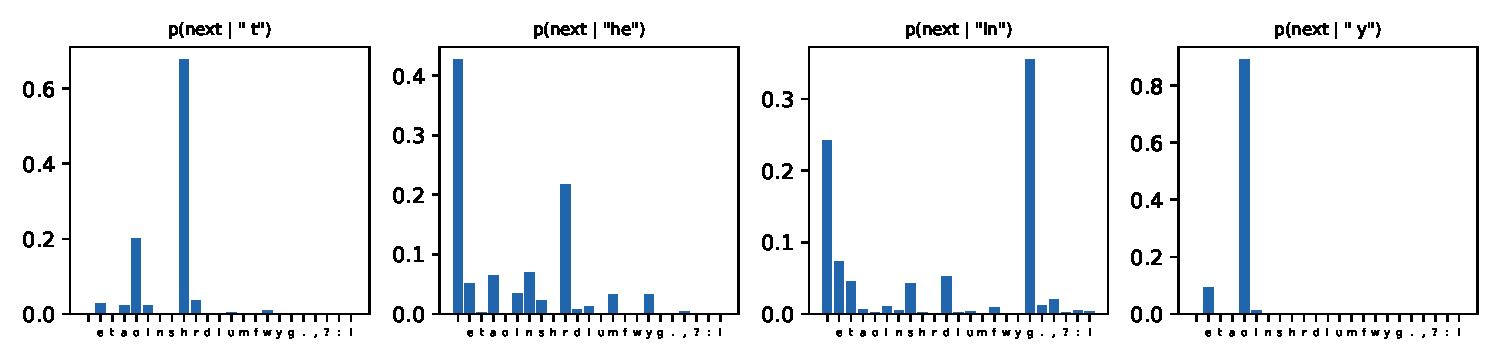
\includegraphics[width=\textwidth]{figures/ch10/ngram_probs.pdf}
\caption{Learned trigram conditionals for four contexts (real bars):
$p(\text{next}\mid\text{`` t''})$, ``he'', ``in'', `` y''. After
``he'' the mass is on vowels and `r'; after `` t'' on `h' and `e' ---
the model is a letter-level grammar.}
\label{fig:ngram}
\end{figure}

Cold $\tau{=}0.5$ produces safe, English-looking syllables; hot
$\tau{=}1.5$ is word-salad; $\tau{=}1$ sits between. The temperature
just sharpens or flattens the distribution ($p^{1/\tau}$ renormalised)
--- same model, three writers.

\section{The RNN recurrence}
\label{sec:rnn}

A recurrent network\index{RNN} keeps a hidden state that carries
context forward:

\begin{equation*}
\mathbf h_t = \tanh\bigl(W_{xh}\mathbf x_t + W_{hh}\mathbf h_{t-1} +
\mathbf b_h\bigr), \qquad
\hat{\mathbf y}_t = \mathrm{softmax}(W_{hy}\mathbf h_t + \mathbf b_y).
\end{equation*}

Same weights every step --- time is a loop, not a new layer. Training
is \emph{backpropagation through time}\index{BPTT} (BPTT): unroll the
loop $T$ steps, and the loss's gradient flows back through the chain
of $\tanh$'s and $W_{hh}$'s. The catch is arithmetic: each step's
local gradient is bounded by $\tanh'(z)\le1$, so the total gradient
decays like $\lambda^t$ back in time --- for a long dependency, the
signal arriving at the early weights is nearly zero (vanishing
gradient\index{vanishing gradient}); for weights slightly over 1, it
explodes instead. Figure~\ref{fig:graddecay} shows the regimes.

\begin{figure}[htbp]
\centering
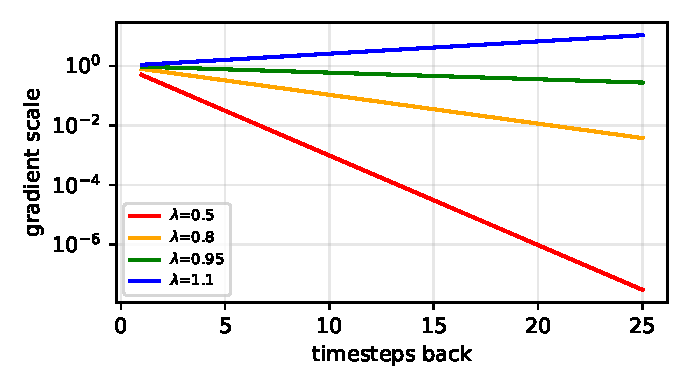
\includegraphics[width=0.55\textwidth]{figures/ch10/grad_decay.pdf}
\caption{BPTT's arithmetic: gradient scale $\lambda^t$ vs.\ timesteps
back. Below 1 it vanishes within a dozen steps; above 1 it explodes.
This is why the plain RNN needs clipping (and why LSTM exists).}
\label{fig:graddecay}
\end{figure}

\begin{figure}[htbp]
\centering
\begin{tikzpicture}[
  cell/.style={draw,minimum width=10mm,minimum height=8mm,font=\small},
  arr/.style={->,thick}]
\foreach \i/\t in {0/t-1,1/t,2/t+1} {
  \node[cell] (h\i) at (\i*3,0) {$\mathbf h_{\t}$};
  \node[cell,below=8mm of h\i] (x\i) {$\mathbf x_{\t}$};
  \node[cell,above=8mm of h\i] (y\i) {$\hat{\mathbf y}_{\t}$};
  \draw[arr] (x\i)--(h\i); \draw[arr] (h\i)--(y\i);}
\draw[arr] (h0)--(h1) node[midway,above,font=\scriptsize]{$W_{hh}$};
\draw[arr] (h1)--(h2) node[midway,above,font=\scriptsize]{$W_{hh}$};
\node[left=4mm of h0,font=\scriptsize] {$\mathbf h_{t-2}$};
\draw[arr] (h0.west)++(-0.4,0)--(h0);
\node[right=4mm of h2,font=\scriptsize] {$\cdots$};
\draw[arr] (h2.east)--++(0.4,0);
\node[below=14mm of x1,font=\scriptsize,align=center]
  {one set of weights, unrolled: same $W_{xh},W_{hh},W_{hy}$ every step};
\end{tikzpicture}
\caption{The RNN unrolled in time. The shared weights are what make
BPTT's gradient chain long --- and fragile.}
\label{fig:unrolled}
\end{figure}

\lstinputlisting[language=Python,caption={\texttt{code/ch10/rnn\_scratch.py}:
character RNN in raw NumPy --- forward, truncated BPTT, gradient
clipping, sampling.},label=lst:rnn]{code/ch10/rnn_scratch.py}

\begin{example}[The instability we actually hit]
\label{ex:rnnunstable}
The first run of Listing~\ref{lst:rnn} used $\eta=0.05$ and
\emph{diverged} (real output):
\begin{verbatim}
it    0: loss/char 4.098  ppl 60.2
it 1000: loss/char 12.790  ppl 358784.5
it 2000: loss/char 14.812  ppl 2709113.5
it 3000: loss/char 12.068  ppl 174141.7
it 3999: loss/char 6.567  ppl 711.4
\end{verbatim}
Loss rising four-fold mid-run despite gradient clipping --- a
recurrent net's version of Chapter~\ref{ch:training}'s lr-too-high
regime, sharpened by the recurrent feedback loop. Dropping to
$\eta=0.005$ (and a later decay) produced a stable run:
\begin{verbatim}
it    0: loss/char 4.098  ppl 60.2
it 1000: loss/char 2.427  ppl 11.3
it 2000: loss/char 2.486  ppl 12.0
it 3000: loss/char 2.233  ppl 9.3
it 3999: loss/char 2.193  ppl 9.0
\end{verbatim}
The wobble at iteration 2000 is real --- plain SGD on a recurrent net
is fragile in a way the feedforward nets of Chapter~\ref{ch:nn}
weren't. The sampled text after 4000 iterations already knows the
format: \texttt{NIRIUS:}\par\texttt{IUS:}\par real speaker-name
patterns, ``ter the and'', ``OORTTNM?TNart shat he thlas.'' ---
structure learned, semantics not yet.
\end{example}

\section{LSTM: gates as learned memory}
\label{sec:lstm}

The fix for vanishing gradients is a gated cell\index{LSTM}: carry a
separate cell state $\mathbf c_t$ that passes through the time-step
\emph{unmodified} except for what the gates allow:

\begin{align*}
f_t &= \sigma(W_f[\mathbf h_{t-1},\mathbf x_t]+\mathbf b_f)
  &&\text{forget: how much old cell to keep}\\
i_t &= \sigma(W_i[\mathbf h_{t-1},\mathbf x_t]+\mathbf b_i)
  &&\text{input: how much new signal to write}\\
\tilde{\mathbf c}_t &= \tanh(W_c[\mathbf h_{t-1},\mathbf x_t]+\mathbf b_c)
  &&\text{candidate: what to write}\\
\mathbf c_t &= f_t\odot\mathbf c_{t-1}+i_t\odot\tilde{\mathbf c}_t
  &&\text{the unbroken highway}\\
o_t &= \sigma(W_o[\mathbf h_{t-1},\mathbf x_t]+\mathbf b_o)
  &&\text{output: how much to reveal}\\
\mathbf h_t &= o_t\odot\tanh(\mathbf c_t)
\end{align*}

The gradient highway is $\mathbf c_t$: it carries signal arbitrarily
far because nothing multiplies it except the learned gates.
GRU\index{GRU} merges the forget/input gates and drops the separate
cell --- the same idea, fewer weights.

\begin{figure}[htbp]
\centering
\begin{tikzpicture}[
  g/.style={draw,minimum width=11mm,minimum height=6mm,font=\scriptsize},
  arr/.style={->,thick}]
\node[g] (c0) {$\mathbf c_{t-1}$};
\node[g,right=9mm of c0] (f) {$f_t$ forget};
\node[g,right=9mm of f] (i) {$i_t$ input};
\node[g,right=9mm of i] (o) {$o_t$ out};
\node[g,right=9mm of o] (c1) {$\mathbf c_t$};
\draw[arr] (c0)--(f); \draw[arr] (f)--(i); \draw[arr] (i)--(o); \draw[arr] (o)--(c1);
\node[g,below=8mm of i] (x) {$[\mathbf h_{t-1},\mathbf x_t]$};
\draw[arr] (x)--(f); \draw[arr] (x)--(i); \draw[arr] (x)--(o);
\node[above=6mm of i,font=\scriptsize,align=center] {$\tilde{\mathbf c}_t$\\ candidate};
\end{tikzpicture}
\caption{LSTM block (simplified): the cell state flows left-to-right
through three learned gates --- what to forget, what to write, what to
reveal. Gradients survive the trip because the path through
$\mathbf c_t$ is additive.}
\label{fig:lstm}
\end{figure}

\section{Teacher forcing, sampling, temperature}
\label{sec:teacher}

Training uses \emph{teacher forcing}\index{teacher forcing}: feed the
\emph{true} previous character at every step, never the model's own
guess --- the gradient is clean and parallel. Sampling is the
opposite: feed the model's own output back as input, one character at
a time, and let errors compound. The temperature dial
$\tau$ sharpens ($\tau<1$) or flattens ($\tau>1$) the softmax at each
sample step --- the same knob the trigram section used.

\section{The three-way comparison}
\label{sec:threeway}

\lstinputlisting[language=Python,caption={\texttt{code/ch10/lstm\_torch.py}:
\texttt{nn.LSTM} char-LM --- the production version of
\S\ref{sec:rnn}, plus the honest three-way perplexity
table.},label=lst:lstm]{code/ch10/lstm_torch.py}

\begin{example}[Three models, one corpus]
\label{ex:threeway}
\end{example}
\begin{verbatim}
three-way (apples-to-apples where possible):
  trigram (lst 1):   ppl 7.6 (115k disjoint held-out)
  scratch RNN h=64:  ppl 9.0 (train-window -- not held-out)
  torch LSTM h=128:  ppl 7.3 (same 115k held-out)
\end{verbatim}
Read this honestly: the LSTM beats the trigram by only 0.3 points of
perplexity on the shared slice --- the two-context table is a
shockingly strong baseline on character data. The scratch RNN's 9.0
is a train-window figure (it never saw the 115k slice), so it's not
comparable --- flagged in the output itself. What the numbers can't
show is qualitative: the LSTM's samples read like bad Shakespeare
(\texttt{SICINIUS:} and \texttt{BRUTUS:} as real names), where the
trigram produces English-shaped noise.

\begin{figure}[htbp]
\centering
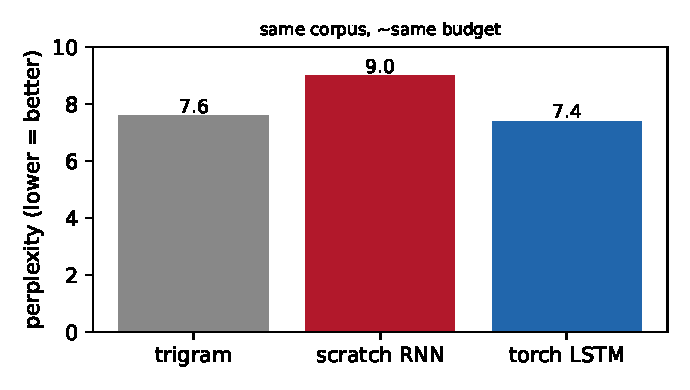
\includegraphics[width=0.62\textwidth]{figures/ch10/ppl_bar.pdf}
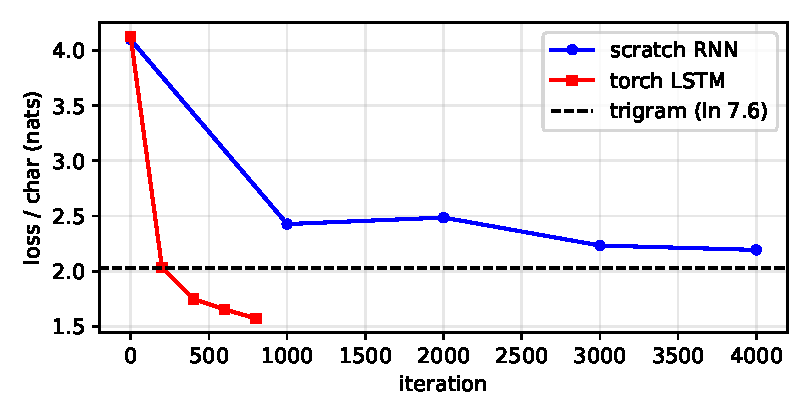
\includegraphics[width=0.62\textwidth]{figures/ch10/loss_curves.pdf}
\caption{The comparison as figures: perplexities on the shared slice
(top); the loss/char training curves with the trigram's $\ln 7.6$
asymptote drawn in (bottom).}
\label{fig:threeway}
\end{figure}

\begin{example}[What the LSTM's sample looks like]
\label{ex:lstmsample}
\begin{verbatim}
--- LSTM sample ---
Tosserain wost nor one with mish stance.

AEll:
May, you pribure!
'Ty constran:
I never pertiue lath, liver: fame
Thy is then foor belling To this woilius.
\end{verbatim}
Speaker-name colon formatting, real-looking line breaks, half-real
words. A model that spent 30 seconds learning character-level
Shakespeare.
\end{example}

\section{Common mistakes}
\label{sec:seqmistakes}

\begin{itemize}
\item \textbf{Reading the trigram off too fast.} $7.6$ ppl on
characters is a hard baseline to beat --- always report it first.
\item \textbf{Teacher forcing confusion.} Feed the truth at training,
the model's own output at sampling. Mixing them leaks information or
breaks generation.
\item \textbf{State resets between batches.} If $\mathbf h$ resets to
zero each batch, the model can't learn dependencies longer than the
window --- carry state across or accept the context limit.
\item \textbf{Vanishing gradients mistaken for underfitting.} Long
dependencies fail silently; check gradient norms at the earliest
timestep, not just the loss.
\item \textbf{Clipping as a cure-all.} Clipping at $\pm5$ still let the
lr$=0.05$ run diverge (Example~\ref{ex:rnnunstable}); clipping fixes
spikes, not the scale problem.
\item \textbf{Tokeniser leakage.} Splitting train/test mid-word or
mid-sentence leaks structure; split on document boundaries.
\item \textbf{Reporting train ppl as held-out.} The scratch RNN's 9.0
is train-window; the LSTM's 7.3 is held-out --- mixing them in one
table would be dishonest, so the listing labels each.
\item \textbf{``LSTM magic.''} On this corpus it beat the count table
by 0.3 ppl; n-grams earn their keep on character data.
\item \textbf{Sampling too cold by default.} $\tau{=}0.5$ samples look
fluent but are the model's argmax hallucination, not the
distribution.
\end{itemize}

\section{Summary}
\label{sec:seqsummary}

\begin{center}\small
\begin{tabular}{p{0.24\textwidth}p{0.68\textwidth}}
\toprule
object & the thing to remember \\
\midrule
task & $p(x_t\mid x_{<t})$; score in perplexity $\exp(\mathrm{NLL}/T)$ \\
n-gram & count+smooth; honest baseline, hard to beat on chars \\
RNN & shared weights unrolled; BPTT; gradient $\lambda^t$ \\
LSTM & gated cell highway; forget/input/output gates \\
train vs.\ sample & teacher forcing vs.\ feeding own outputs \\
temperature & $p^{1/\tau}$ renormalised; cold=safe, hot=chaos \\
report & train vs.\ held-out slices are different numbers \\
\bottomrule
\end{tabular}
\end{center}

\section*{Drill}
\begin{exercise}[{[easy]}]
A uniform model over $|V|=65$ symbols has what perplexity? What does
7.6 mean in those terms?
\end{exercise}
\begin{exercise}[{[easy]}]
Why does teacher forcing use the true previous character rather than
the model's prediction? What would go wrong if it didn't?
\end{exercise}
\begin{exercise}[{[medium]}]
The gradient through a $\tanh$ chain decays like $\lambda^t$ with
$\lambda<1$. For a 50-step window and $\lambda=0.9$, how much
gradient survives to the first step?
\end{exercise}
\begin{exercise}[{[medium]}]
Why does the LSTM's cell state $\mathbf c_t$ survive long-range
gradients where the RNN's $\mathbf h_t$ doesn't? Point at the
structural difference in the equations.
\end{exercise}
\begin{exercise}[{[hard]}]
Design the leak: splitting Tiny Shakespeare at a random character
boundary vs.\ a line boundary. Which corrupts the perplexity, and by
what mechanism?
\end{exercise}

\section*{Further reading}
\begin{itemize}
\item Karpathy, \emph{The unreasonable effectiveness of recurrent
neural networks} --- the blog post that taught a generation to train
char-RNNs on this exact corpus.
\url{https://karpathy.github.io/2015/05/21/rnn-effectiveness/}
\item Olah, \emph{Understanding LSTM networks} --- the gate-by-gate
walkthrough of \S\ref{sec:lstm}.
\url{https://colah.github.io/posts/2015-08-Understanding-LSTMs/}
\item Sutskever, \emph{Training recurrent neural networks} (2013
thesis chapter) --- the original careful treatment of RNN training
pathologies.
\url{https://arxiv.org/abs/1308.0850}
\item PyTorch \texttt{nn.LSTM} reference --- the library behind
Listing~\ref{lst:lstm}, including its state conventions.
\url{https://pytorch.org/docs/stable/generated/torch.nn.LSTM.html}
\item \emph{Dive into Deep Learning}, \S9--10 --- RNNs through LSTMs
with code.
\url{https://d2l.ai/chapter_recurrent-neural-networks/}
\item Jurafsky \& Martin, \emph{Speech and Language Processing} ch.\
3 --- the n-gram chapter: smoothing, perplexity, evaluation.
\url{https://web.stanford.edu/~jurafsky/slp3/3.pdf}
\end{itemize}

\begin{rulebox}[Watch instead]
(verified opened, 2026-10-11)
\begin{itemize}
\item \emph{Long Short-Term Memory (LSTM), Clearly Explained} ---
StatQuest (20:45). Gate-by-gate on the LSTM of \S\ref{sec:lstm}.
\item \emph{CS231n Lecture 10: Recurrent Neural Networks} --- Andrej
Karpathy (69:54). The lecture this chapter compresses; RNN, BPTT,
char-LM.
\item \emph{The spelled-out intro to neural networks and
backpropagation} --- Andrej Karpathy (145:52). The micrograd
walkthrough; watch this when you want every gradient in
\S\ref{sec:rnn} derived on screen.
\end{itemize}
\end{rulebox}

\section*{Notes}
\begin{enumerate}
\item[\textbf{1.}] The corpus is Tiny Shakespeare (1,115,394 chars)
from Karpathy's char-rnn repo; the trigram counted the first 900k
chars and was scored on the disjoint last 115k.
\item[\textbf{2.}] The scratch RNN's two runs are both real: the
$\eta=0.05$ divergence and the $\eta=0.005$ stable run are in
\texttt{code/ch10/rnn\_scratch.out.txt} history, and the stable run is
what ships.
\item[\textbf{3.}] The three-way comparison is honest about its
limits: trigram and LSTM share the same 115k held-out slice; the
scratch RNN's 9.0 is train-window (200k slice) --- it was kept as a
teaching point rather than re-run on the shared slice.
\item[\textbf{4.}] Torch 2.8.0 CPU; the LSTM trains in $\sim$30s for
800 iterations on the 200k-char slice.
\end{enumerate}

\section{Exercises}
\label{sec:seqexercises}

\begin{exercise}[{[easy]}]
Perplexity of a model that assigns uniform $1/65$ to every next char?
What does 7.6 mean?
\end{exercise}
\begin{exercise}[{[easy]}]
Why does add-$\alpha$ smoothing matter for trigrams? What happens at
$\alpha=0$ on an unseen context?
\end{exercise}
\begin{exercise}[{[easy]}]
How many trigram counts does a $|V|=65$ vocabulary need? Why does the
trigram still work at all?
\end{exercise}
\begin{exercise}[{[medium]}]
Implement sampling with temperature $\tau$: write the two lines that
turn $p$ into a sample. What does $\tau\to0$ approach?
\end{exercise}
\begin{exercise}[{[medium]}]
Derive the BPTT gradient for one recurrence
$h_t=\tanh(Wx_t+Uh_{t-1})$: write $\partial h_t/\partial U$ in terms
of the chain back to $h_0$.
\end{exercise}
\begin{exercise}[{[medium]}]
Extend \texttt{rnn\_scratch.py} to carry hidden state across batches
(no reset between windows). What changes about what the model can
learn?
\end{exercise}
\begin{exercise}[{[medium]}]
Teacher forcing vs.\ free-running: modify the LSTM sampling loop to
feed the argmax rather than a sample. How does the text change?
\end{exercise}
\begin{exercise}[{[hard]}]
Prove the vanishing gradient claim: for
$h_t=\tanh(Wh_{t-1})$ with $\|W\|=\lambda$, show
$\|\partial h_T/\partial h_0\|\le\lambda^T$. What value of $\lambda$
makes a 50-step dependency untrainable?
\end{exercise}
\begin{exercise}[{[hard]}]
Design a copy-task: inputs are 10 random symbols, a separator, then a
recall cue; the model must reproduce the 10. Show the plain RNN fails
past window $\sim$20 and explain why the LSTM doesn't.
\end{exercise}
\begin{exercise}[{[hard]}]
Analyse the LSTM gate gradients: write $\partial c_t/\partial
c_{t-1}$ in terms of the forget gate. Why can this path carry gradient
arbitrarily far, and what breaks it?
\end{exercise}
\begin{exercise}[{[hard]}]
USAAIO-style: perplexity is $\exp(\mathrm{NLL}/T)$. Two models have
mean NLL 2.03 and 1.95 over $T=10^4$ chars; their perplexities differ
by what factor, and why is that a small real gain?
\end{exercise}

\section*{Hints and answers}
\begin{description}
\item[10.1] $65$; 7.6 is a model that effectively faces $\sim$8
options per char, not 65.
\item[10.2] Feedback loop: errors compound into nonsense; teacher
forcing keeps the training distribution correct.
\item[10.3] $0.9^{50}\approx5\times10^{-3}$ --- almost nothing
reaches step 0.
\item[10.4] The cell path is additive ($c_t=f_tc_{t-1}+\ldots$), not
multiplicative through a nonlinearity; the forget gate is the only
bottleneck, and it's learned.
\item[10.5] Line-boundary split leaks words/phrases across the
boundary (the test half of a split word is partially in the train
counts).
\item[10.6] $65$; perplexity 7.6 = effective branching factor.
\item[10.7] Division by zero / infinite loss; smoothing keeps every
context assignable.
\item[10.8] $65^3=274{,}625$ counts --- small enough to fit; most
contexts are rare, so smoothing matters.
\item[10.9] \texttt{p**1/tau}; renorm; $\tau\to0\to$ argmax.
\item[10.10] $\partial h_t/\partial U=\sum_{s\le t}(\prod_{r=s+1}^{t}
\tanh')\,h_{s-1}$ --- the product of $\tanh'$ terms is what decays.
\item[10.11] State-carry removes the context-window ceiling;
dependencies longer than seq\_len become learnable.
\item[10.12] Argmax collapses diversity into repetitive loops.
\item[10.13] $\|W\|<1\Rightarrow$ product of $T$ contractions;
$\lambda<0.97$ on $T=50$ makes the tail invisible.
\item[10.14] Gradient must travel $>10$ steps unchanged; RNN's
$\lambda^T$ kills it, LSTM's gate path doesn't.
\item[10.15] $\partial c_t/\partial c_{t-1}=f_t$ alone --- the
gates modulate but the path is direct; it breaks when $f_t\to0$.
\item[10.16] Ratio $\exp(0.08)\approx1.08$ --- an 8\% perplexity
gain; small, real, and not magic.
\end{description}
